
\section{Preliminary}
\label{sec:preli}

\textbf{Labeled Transition Systems (LTS).} 
We use LTS to model behaviors of smart contracts. 
A LTS $A=(Q,\Sigma,  \mathsf{q}_0, \delta)$ over the possibly-infinite alphabet
$\Sigma$ is a possibly-infinite set $Q$ of states with
an initial state $\mathsf{q}_0 \in Q$, and a transition relation $\delta \subseteq Q \times \Sigma \times
Q$. 

\noindent
\textbf{Execution.} 
An \emph{execution} of $A$ is a sequence of states and transition labels (\emph{actions}) $\rho = \mathsf{q}_0, \mathsf{a}_0,\mathsf{q}_1\ldots \mathsf{a}_{k-1},\mathsf{q}_k$ for $k>0$ such that $\delta(\mathsf{q}_i, \mathsf{a}_i, \mathsf{q}_{i+1})$ for each $0\leq i<k$. We write $\mathsf{q}_i\xrightarrow{\mathsf{a}_i\ldots \mathsf{a}_{j-1}}_A \mathsf{q}_j$ to denote the subsequence $\mathsf{q}_i,\mathsf{a}_i,...,\mathsf{q}_{j-1},\mathsf{a}_{j-1},\mathsf{q}_j$ of $\rho$.


% \noindent
% \textbf{Trace.} 
% The projection $\tau| \Gamma$ of a sequence $\tau$ is the maximum subsequence of $\tau$ over the alphabet $\Gamma$.
% A \emph{trace} of $A$ is the projection $\rho | \Sigma$ of an execution $\rho$ of $A$.
% The set of traces of an LTS $A$ is denoted by $\mathit{T}(A)$.

% The $i$th symbol of a sequence $\tau \in \Sigma^*$ is denoted $\tau_i$, and $\epsilon$ is the empty
% sequence ($\mathsf{q}_i\xrightarrow{\epsilon}\mathsf{q}_i$). A transaction is interpreted as an LTS whose traces represent sequences of invocations to a smart contract's methods together with their inputs parameters and outcomes. 



%Typical examples of observable outcomes are the changes on the native token balances of blockchain accounts and the return value, which can be read through invocations from other contracts. 
%The states of a smart contract LTS are composed of an \emph{internal} part represented as assignments to the contract's fields and the balance of the address at which the contract is deployed, and an \emph{environment} part represented as assignments to environment variables, e.g., {\tt now}, which influence the contract's behavior. The transitions represent invocations to the contract's methods or updates of the environment variables, e.g., increasing the value of {\tt block.timestamp}. This LTS can be thought of as a composition between an LTS defining the evolution of the variables controlled by the contract and an LTS defining the evolution of the environment variables (whose states are valuations of these variables). The states of the two LTSs share the valuation of the environment variables (read by the first LTS and updated by the second). The labels record method names, arguments, and observable outcomes. For uniformity, updates of environment variables are modeled as invocations to some fictitious methods. 



\noindent
\textbf{Invocation Label.} 
Formally, an \emph{invocation label} $\adr.m(\vec{u})$ consists of a method name $m$ of a contract address $\adr$, accompanied by a vector $\vec{u}$ containing argument values.

\noindent
\textbf{Operation Label.} 
An \emph{operation label} $\ell :=
\adr.m(\vec{u}) \Rightarrow (I,v) \ \cup\ \bot$ is an invocation label $\adr.m(\vec{u})$ along with a
return value $v$ % \in \vals$ 
, and $I$ is a sequence of operation labels representing the ``internal'' calls made during the invocation of $m$. 
% e.g., an internal call to {\tt send} Ether. 
% $\vals$ is the domain of argument or return values. 
The distinguished invocation outcome $\bot$ is associated to invocations that revert. 


\noindent
\textbf{Interface.}
% We use $\inv{\ell}$ to refer to the invocation label in an operation label $\ell$. This notation is extended to sequences of operation labels. 
The \emph{interface} $\Sigma_{\adr}$ is the set of non-read-only operation labels in the contract $\adr$. We assume w.l.o.g. that the preconditions are satisfied for all the operations in $\Sigma_{\adr}$, otherwise, the external invocation $\adr.m(\vec{u})$ reverts. $\Sigma_{\adr}$ is a superset of the set of action candidates of {\name}.  


% We use $\Sigma_{\adr}^{\checkmark}$ to denote the subset of $\Sigma_{\adr}$ that excludes operation labels with $\bot$ as a return value, and $\meths{\Sigma_{\adr}}$ to denote the method names in $\Sigma_{\adr}$. 

\noindent
\textbf{Smart Contract.}
A \emph{smart contract} at an address $\adr$ is an LTS $C_{\adr}=(Q_{\adr},\Sigma_{\adr}, \mathsf{q}_0, \delta_{\adr})$ over the interface $\Sigma_{\adr}$ where $Q_{\adr}$ is the set states and $\delta_{\adr}$ is the transition relation.


% For uniformity to model accounts that are not associated with smart contracts we use the following LTS 
% $C_{\adr}=(Q_{\adr},\{\adr.\send(\adr',u) \Rightarrow (\{\adr'.\send(u) \Rightarrow \mytrue\}, \mytrue)\ \cup\ \bot; \adr.\send(u) \Rightarrow \mytrue; \adr.\bal \Rightarrow v\}, \mathsf{q}_0, \delta_{\adr})$.  The above LTS only contains the native token transfer operation labels and a read-only method to fetch the account native token balance. Note that invocations to read-only methods do not change the state. The invocation label $\adr.\send(\adr',u)$ transfer an amount $u$ of native tokens from the account $adr$ to the account $\adr'$. The outcome is either revert or successful transfer consist of $adr$ local state modification, removing the $u$ amount from its balance, and the operation $\adr'.\send(u) \Rightarrow \mytrue$ that modifies the local state of $\adr'$, adding the $u$ amount to its balance. 



% \begin{definition}
% \textbf{(Evolution)}
% We use $Q = \bigcup\limits_{\adr \in \mathbf{A}} Q_{\adr}$, $\Sigma = \bigcup\limits_{\adr \in \mathbf{A}} \Sigma_{\adr}$, $\delta = \bigcup\limits_{\adr \in \mathbf{A}} \delta_{\adr}$, where $\mathbf{A}$ is the set of all addresses in the blockchain.  We define the LTS $B = (Q,\Sigma,\mathsf{q}_0,\delta)$ to represent the evolution of the whole blockchain state where $\mathsf{q}_0 \in Q$ is the initial state of the blockchain. 
% \end{definition}


\noindent
\textbf{Symbolic Actions Vector.}
We define the notion of a symbolic actions vector $\symbolic = \ell_{\adr 1} \ldots \ell_{\adr n}$ s.t.  $\ell_{\adr i}\in \Sigma$ for $1\leq i<n$ as the sequence of operation labels (possibly from different  contracts) associated with the execution $\rho$, i.e., $\rho = \mathsf{q}_1, \ell_{\adr 1},\mathsf{q}_1\ldots \ell_{\adr n},\mathsf{q}_n$. 
 


% A \emph{symbolic actions vector} is a sequence of operation labels $\symbolic = \ell_{\adr 1} \ldots \ell_{\adr n}$ s.t.  $\ell_{\adr i}\in \Sigma$ for $1\leq i<n$ associated with the execution of $B$  $\rho = \mathsf{q}_1, \ell_{\adr 1},\mathsf{q}_1\ldots \ell_{\adr n},\mathsf{q}_n$ where $\delta(\mathsf{q}_i, \ell_{\adr i}, \mathsf{q}_{i+1})$ for $1\leq i<n$.



% We use $\mathbf{T}$ to denote the domain of tokens identifiers (including native token). 
% We define the mapping $\tokenmap:  Q \times \mathbf{A} \times  \mathbf{T} \implies \mathbf{V}$ that maps the tuple $(\mathsf{q},\adr,\mathsf{t}) \in Q \times \mathbf{A} \times \mathbf{T}$ consisting of a blockchain state, an address, a token identifier, to the amount of token $\mathsf{t} \in \mathbf{T}$ holds by the address $\adr \in \mathbf{A}$ at the blockchain state $\mathsf{q} \in Q$. We define the mapping $\tokenpricemap: \mathbf{T} \implies \mathbf{V}$ that maps each token $\mathsf{t}$ to its price. 


\noindent
\textbf{Balance.} 
We define the balance of address $\adr$ in a blockchain state $\mathsf{q}$ as the mapping $\Balance: Q \times \mathbf{A} \implies \mathbf{V}$
    that maps the pair $(\mathsf{q},\adr) \in Q \times \mathbf{A}$ to the weighted sum of tokens the address $\adr$ holds at $\mathsf{q}$, i.e., 
    $\Balance(\mathsf{q},\adr)= \sum_{\mathsf{t} \in \mathbf{T}}{\tokenmap(\mathsf{q},\adr,\mathsf{t}) \cdot \tokenpricemap(\mathbf{t})}$, where $\mathbf{T}$ represents tokens hold by $\adr$, $\tokenmap(\mathsf{q},\adr,\mathsf{t})$ represents the amount of token $\mathsf{t}$ hold by $\adr$ at the blockchain state $\mathsf{q}$, and $\tokenpricemap(\mathsf{q}, \mathbf{t})$ represents the price of token $\mathsf{t}$ at the blockchain state $\mathsf{q}$.


%The value of a balance state $\Balance = (\tokenset, \tokenmap)$ is defined as the weighted sum $\sum_{\token \in \tokenset}{\tokenmap(\token) \cdot \tokenpricemap(\token)}$.

% Next we define an attack vector by an address $\adr$ as a symbolic actions vector $\symbolic$ where the symbolic arguments of a method invocation are replaced with concrete values (integer values) and $\symbolic$ transforms a blockchain state $\mathsf{q}$ to another state $\mathsf{q}'$ such that $\Balance(\mathsf{q}',\adr) -  \Balance(\mathsf{q},\adr) > 0$, i.e., the adversary $\adr$ is able to generate profit when the sequence of actions $\symbolic$ is executed with the concrete values. 

%\begin{definition}[Profit]
%\label{profit}
%Given the initial balance state(before exploit) $\Balance_0$ and the final state(after exploit) $\Balance_n$, the adversarial profit $\profit(\Balance_0, \Balance_n)$ is defined as the increase of the values of balance states: $\profit(\Balance_0, \Balance_n) = \sum_{\token \in \tokenset_n}{\tokenmap(\token) \cdot \tokenpricemap(\token)} - \sum_{\token \in \tokenset_0}{\tokenmap(\token) \cdot \tokenpricemap(\token)}$.
%\end{definition}
%
%
\noindent
\textbf{Attack Vector.}
    An \emph{attack vector} by an adversary $\adr$ consists of a symbolic actions vector $\symbolic$ where the symbolic arguments are replaced by concrete values (integer values) and $\symbolic$ transforms a blockchain state $\mathsf{q}$ to another state $\mathsf{q}'$ such that $\Balance(\mathsf{q}',\adr) -  \Balance(\mathsf{q},\adr) > 0$, i.e., the adversary $\adr$ generates profit when the sequence of actions $\symbolic$ is executed with the concrete values. 


%Given a set of possible actions, we are interested in synthesizing the right sequence of actions and their optimal parameters to maximize an adversary's profit. During the synthesis procedure, in different stages, an attack vector has different forms depending on its completeness. 


%\begin{definition}[Partial Attack Vector]
%\label{def:attackvector}
%A partial attack vector is a sequence of actions with some actions represented as holes($?$) and all parameters represented as symbolic values($a, b, c, ...$).  
%\end{definition}


%\begin{definition}[Concrete Attack Vector]
%\label{def:concrete}
%A concrete attack vector $\concrete$ for a symbolic attack vector $\symbolic$ replaces each symbolic argument to a function call with a concrete integer. $\paras$ is the corresponding parameter vector.
%\end{definition}

%In the remainder of this paper, given an attack vector $\attackvector$, we write $IsPartial(\attackvector)$, $IsSymbolic(\attackvector)$, and $IsConcrete(\attackvector)$ to denote $\attackvector$ is a partial/symbolic/concrete attack vector respectively. 

% \vspace{-1.5mm}
% \begin{example}
% The following is a symbolic actions vector generated during the synthesis of Harvest USDC attack.
% \end{example}
% \vspace{-7.5mm}
% \begin{align*}  
% \codeword{deposit(v)} \cdot \codeword{exchange(USDC, USDT, v)}\ \cdot \\
% \codeword{withdraw(v)}  \cdot \codeword{exchange(USDT, USDC, v)}
% \end{align*} 
% \vspace{-0.5mm}
% \noindent  \emph{The following attack vector is one concretization of the above symbolic} \emph{actions vector given by {\name}, 
% which yields $1767$ USD profit.}
% \vspace{-1mm}
% \begin{align*}  
% \codeword{deposit(42989457)} \cdot \codeword{exchange(USDC, USDT,  6957833)}\ \cdot \\
% \codeword{withdraw(43866454)}\ \cdot \codeword{exchange(USDT, USDC, 9550781)}
% \end{align*} 
% \vspace{-5mm}


 %The state transition of a concrete attack vector can be expressed as sequential transitions of individual actions. Formally,
 
%$$(\pstate_0,\Balance_0)\xrightarrow[]{\transit(p_0, p_1, ..., p_n)}(\pstate_{n+1}, \Balance_{n+1}) \Leftrightarrow (\pstate_0,\Balance_0)\xrightarrow[]{\transit_0(p_0)}(\pstate_1, \Balance_1)\xrightarrow[]{\transit_1(p_1)}...\xrightarrow[]{\transit_n(p_n)}(\pstate_{n+1}, \Balance_{n+1})$$
 
%\subsection{Problem Statement}
\noindent
\textbf{Problem formulation.}
Given a specification $\spec$ (which contains vulnerable contract addresses or action candidates) and a blockchain state $\mathsf{q}$, the objective is to find an attack vector consisting of a concretization of the symbolic actions vector $\symbolic = \ell_{\adr 1} \ldots \ell_{\adr n}$ s.t.  $\ell_{\adr i}\in \Sigma \cap \spec$  for $1\leq i<n$, transforming the state $\mathsf{q}$ to a state $\mathsf{q}'$, and that maximizes the profit of an adversary $\adr$, $\Balance(\mathsf{q}',\adr) -  \Balance(\mathsf{q},\adr)$. 


%The synthesis task can be divided into two sub-tasks. (1) Synthesize all profitable symbolic attack vector $\symbolic$ from the specification $\spec$. (2) Find the optimal parameters for the concrete attack vector $\concrete$ to yield the maximum profit. Figure ~\ref{fig:attackvectorflow} shows different forms of attack vectors during different stages of our synthesis process. 
 

%\begin{figure}
%    \centering
%    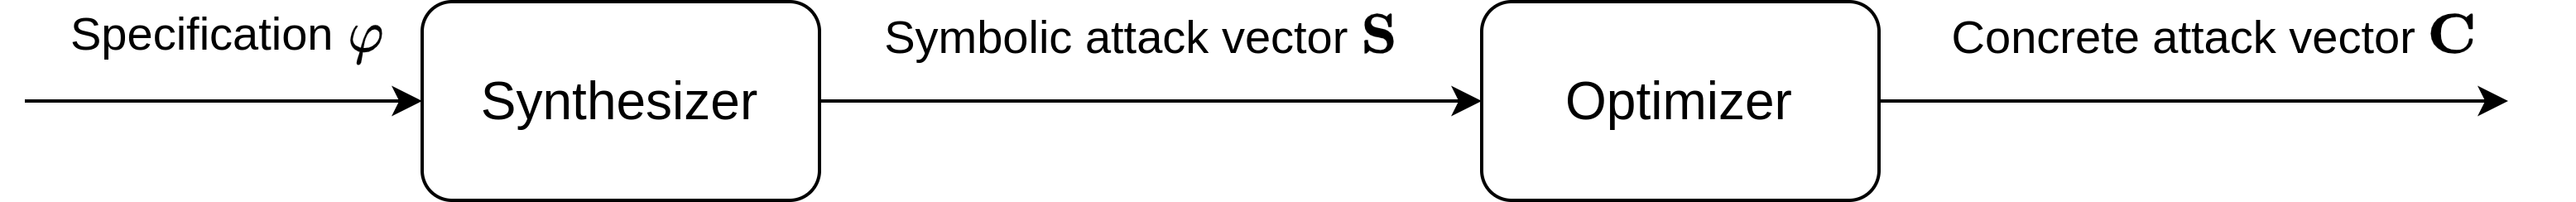
\includegraphics[width=\linewidth]{figures/attackvectorflow.png}
%    \caption{Different forms of attack vectors during synthesis process}
%    \label{fig:attackvectorflow}
%\end{figure}

